%%%%%%%%%%%%%%%%%%%%%%%%%%%%%%%%%%%%%%%%%%%%%%%%%%%%%%%%%%%%%%%%%%%%%%%%%%%%%
%% Original default rstudio/pandoc latex file
%% upated by @jhollist 09/15/2014
%% inspired by @cboetting https://github.com/cboettig/template and
%% @rmflight blog posts:
%% http://rmflight.github.io/posts/2014/07/analyses_as_packages.html 
%% http://rmflight.github.io/posts/2014/07/vignetteAnalysis.html).  
%%%%%%%%%%%%%%%%%%%%%%%%%%%%%%%%%%%%%%%%%%%%%%%%%%%%%%%%%%%%%%%%%%%%%%%%%%%%%

\documentclass[11pt,a4paper]{article}
\usepackage[T1]{fontenc}
\usepackage{lmodern}
\usepackage{amssymb,amsmath}
\usepackage{ifxetex,ifluatex}
\usepackage{fixltx2e} % provides \textsubscript
% use upquote if available, for straight quotes in verbatim environments
\IfFileExists{upquote.sty}{\usepackage{upquote}}{}
\ifnum 0\ifxetex 1\fi\ifluatex 1\fi=0 % if pdftex
  \usepackage[utf8]{inputenc}
\else % if luatex or xelatex
  \ifxetex
    \usepackage{mathspec}
    \usepackage{xltxtra,xunicode}
  \else
    \usepackage{fontspec}
  \fi
  \defaultfontfeatures{Mapping=tex-text,Scale=MatchLowercase}
  \newcommand{\euro}{€}
\fi
% use microtype if available
\IfFileExists{microtype.sty}{\usepackage{microtype}}{}
\usepackage[margin=1in]{geometry}
\usepackage{longtable,booktabs}
\usepackage{graphicx}
% Redefine \includegraphics so that, unless explicit options are
% given, the image width will not exceed the width of the page.
% Images get their normal width if they fit onto the page, but
% are scaled down if they would overflow the margins.
\makeatletter
\def\ScaleIfNeeded{%
  \ifdim\Gin@nat@width>\linewidth
    \linewidth
  \else
    \Gin@nat@width
  \fi
}
\makeatother
\let\Oldincludegraphics\includegraphics
{%
 \catcode`\@=11\relax%
 \gdef\includegraphics{\@ifnextchar[{\Oldincludegraphics}{\Oldincludegraphics[width=\ScaleIfNeeded]}}%
}%
\ifxetex
  \usepackage[setpagesize=false, % page size defined by xetex
              unicode=false, % unicode breaks when used with xetex
              xetex]{hyperref}
\else
  \usepackage[unicode=true]{hyperref}
\fi
\hypersetup{breaklinks=true,
            bookmarks=true,
            pdfauthor={},
            pdftitle={working title Compatibility system and stygma size of pollen recipient as main predictors of heterospecific pollen effect},
            colorlinks=true,
            citecolor=blue,
            urlcolor=blue,
            linkcolor=magenta,
            pdfborder={0 0 0}}
\urlstyle{same}  % don't use monospace font for urls
\setlength{\parindent}{0pt}
\setlength{\parskip}{6pt plus 2pt minus 1pt}
\setlength{\emergencystretch}{3em}  % prevent overfull lines
\setcounter{secnumdepth}{0}

%%%%%%%%%%%%%%%%%%%%%%%%%%%%%%%%%%%%%%%%%%%%%%%%%%%%%%%%
%Changes borrowed from @cboettig, added by @jhollist 
% A modified page layout 
\textwidth 6.75in
\oddsidemargin -0.15in
\evensidemargin -0.15in
\textheight 9in
\topmargin -0.5in
\usepackage{lineno} % add 
  \linenumbers % turns line numbering on 
%%%%%%%%%%%%%%%%%%%%%%%%%%%%%%%%%%%%%%%%%%%%%%%%%%%%%%%%

%%%%%%%%%%%%%%%%%%%%%%%%%%%%%%%%%%%%%%%%%%%%%%%%%%%%%%%%
%%Packages and layout changes by @jhollist 09/15/2014
\usepackage{ragged2e}
\usepackage[font=normalsize]{caption}
  \usepackage[doublespacing]{setspace}
\usepackage{parskip}
\usepackage{fancyhdr}
\pagestyle{fancy}
\fancyhf{}
\renewcommand{\headrulewidth}{0pt}
  \rfoot{\today}
\lfoot{\thepage}
%%Changed default abstract width and added lines
\renewenvironment{abstract}{
  \hfill\begin{minipage}{1\textwidth}
  \rule{\textwidth}{1pt}\vspace{5pt}
  \normalsize
  \begin{justify}
  \bfseries\abstractname\vspace{5pt}
  \end{justify}}
  {\par\noindent\rule{\textwidth}{1pt}\end{minipage}
}
%%%%%%%%%%%%%%%%%%%%%%%%%%%%%%%%%%%%%%%%%%%%%%%%%%%%%%%%

\title{working title Compatibility system and stygma size of pollen recipient
as main predictors of heterospecific pollen effect}
\author{
Jose B. Lanuza, Ignasi Bartomeus, Tia-Lynn Ashman, Romina Rader
}
\date{}
% Allowing for landscape pages
\usepackage{lscape}
\newcommand{\blandscape}{\begin{landscape}}
\newcommand{\elandscape}{\end{landscape}}

% Left justification of the text: see https://www.sharelatex.com/learn/Text_alignment
% \usepackage[document]{ragged2e} % already in the latex template
\newcommand{\bleft}{\begin{flushleft}}
\newcommand{\eleft}{\end{flushleft}}

%%Fix tightlist error: https://stackoverflow.com/questions/40438037/tightlist-error-using-pandoc-with-markdown
%%Added 2018-03-26 
\providecommand{\tightlist}{%
  \setlength{\itemsep}{0pt}\setlength{\parskip}{0pt}}
%%%  
  

\begin{document}
%%Edited by @jhollist 09/15/2014
%%Adds title from YAML
\begin{singlespace}
\begin{center}
\huge working title Compatibility system and stygma size of pollen recipient
as main predictors of heterospecific pollen effect
\end{center}
%%Adds Author, correspond email asterisk, and affilnum from YAML
\begin{center}
\large
Jose B. Lanuza, Ignasi Bartomeus, Tia-Lynn Ashman, Romina Rader \textsuperscript{*} \textsuperscript{1,2,3} 
\end{center}
%%Adds affiliations from YAML
\begin{justify}
\footnotesize \emph{ 
\\*
\textsuperscript{1}US Environmental Protection Agency, Office of Research and Development,
National Health and Environmental Effects Research Laboratory, Atlantic
Ecology Division, 27 Tarzwell Drive Narragansett, RI, 02882, USA\\*
\\*
\textsuperscript{2}Big Name University, Department of R, City, BN, 01020, USA\\*
\\*
\textsuperscript{3}Estacion Biologica de Donana (EBD-CSIC), E-41092 Sevilla, Spain\\*
}
%%Adds corresponding author email(s) from YAML
\newcounter{num}
\setcounter{num}{1}
\\[0.1cm]
\footnotesize \emph{ 
\ifnum\value{num}=1%
\textsuperscript{*} corresponding author:
\fi
\href{mailto:barragansljose@gmail.com}{\nolinkurl{barragansljose@gmail.com}}
\stepcounter{num}
}
\end{justify}
%%Adds date from YAML
\normalsize

\end{singlespace}


\singlespace

\vspace{2mm}\hrule

Pollinator sharing can have negative consequences for species fitness
with the arrival of foreign pollen. However, the costs of heterospecific
pollen are not yet well understood. For this reason, we have conducted a
glasshouse experiment where we try to understand how phylogenetic
relatedness and the different traits of these species are involved in
this process. We experimentally crossed 10 species belonging to three
different families: Brassicaceae, Solanaceae and Convolvulaceae.
Overall, more than 4000 crosses were done and seed set and pollen tubes
were considered as proxy of effect. We found that for all species
foreign pollen (50\% or less) reduced seed set. Moreover, the seed set
reduction is not dependent on the degree of relatedness of the pollen
donor. However, the effect is governed by the degree of relatedness and
the traits of the species recipient. Our results show that the outcome
of heterospecific pollen deposition is determined in greater degree by
the traits of the pollen recipient than the pollen donor and that
certain traits such as compatibility system are crucial to understand
the costs of heterospecific pollen.

\vspace{3mm}\hrule

\emph{Keywords}: heterospecific pollen, plant reproduction, fitness,
interspecific competition, phylogenetic distance.

\doublespace

\bleft

\section{INTRODUCTION}\label{introduction}

\textbf{Paragraph 1} General idea to our concept

In most ecosystems, plant species normally coexist and share their
floral visitors with other species Bascompte et al. (2003). From the
plants' perspective, this pollinator sharing can be positive due to
facilitation Carvalheiro et al. (2014) or negative due to competition at
the pre-pollination stage Pauw (2013). An increasing number of visits
often correlates with higher chances of fertilization Engel and Irwin
(2003). However this is not always the case, among these possible flower
visitors there are also nectar robbers and pollen thieves Inouye (1980).
Receiving both sufficient quantity and quality deposited on the stigma
is thus highly relevant to the pollination success of the plant Aizen
and Harder (2007).

\textbf{Paragraph 2} Introducing topic and knowledge gap

By visiting many plant species, many pollinators are responsible for
conspecific pollen loss and the transport of foreign pollen, both of
which can have important detrimental effects on species fitness Morales
and Traveset (2008); Ashman and Arceo-Gómez (2013); Arceo-Gómez and
Ashman (2016). Foreign pollen arrival can play an important role in
plant species fitness but outcomes are variable and appear to be context
dependent as there is not always a decrease in fitness Morales and
Traveset (2008). Some of this variation is likely due to the enormous
variability of foreign pollen transferred across systems ranging from
between 0 and 75 percent but most studies report ranges of
heterospecific pollen between 0 and 20 percent of the total pollen load
Bartomeus et al. (2008) Montgomery and Rathcke (2012); Ashman and
Arceo-Gómez (2013); Fang and Huang (2013), yet even these relatively low
amounts of heterospecific pollen transferred can decrease fitness
greatly Thomson et al. (1982). While we now have some understanding of
the impacts of heterospecific pollen quantity, we have less
understanding of other factors that could be driving the variation in
impacts upon fitness. Ashman and Arceo-Gómez (2013) postulated the first
predictive framework that identifies a need to understand how plant
traits might mediate heterospecific pollen effect, whereby mating system
and pollen size were predicted to potentially mediate the impact of
foreign pollen transfer on plant fitness. This concept is supported by
other studies, such as Tong and Huang (2016) that demonstrate an
asymmetrical effect in 6 species of Pedicularis whereby the pollen of
long styled species was able to grow the full length of the style on
short styled species but not vice versa. While this suggests that the
impacts of heterospecific pollen may differ among pollen donor and
recipient, few studies have been conducted to ascertain whether this
pattern is in fact a trend or to identify the extent to which other
plant traits are critical to heterospecific pollen impacts.

\textbf{Paragraph 3} Expanding ideas with examples

Given the large variability in mating systems across populations
Whitehead et al. (2018), it is difficult to determine potential impacts
upon HP transfer yet incompatibility system is another plant trait that
appears to play an important role in foreign pollen effect whereby
species that are self incompatible have stronger barriers to
heterospecific pollen than self-compatible species Ashman and
Arceo-Gómez (2013). The type of incompatibility, (i.e.~whether
sporophytic or gametophytic) is related to the location of pollen
recognition; sporophytic incompatibility relates to signaling at the
stigma surface while gametophytic occurs within the style. This later
acting pollen recognition mechanism is associated with greater negative
effect than sporophytic recognistion Barrett (1988). Nonetheless, an
effect of foreign pollen is a bit obscured by the variability within
species, however species that are strong selfers or strong outcrossers
have less variablity in mating systems and predictions of effect could
be more realistic (see figure 1 from Whitehead et al. (2018)). Moreover,
other traits such as number of pollen grains per flower and number of
ovules have been traditionally associated with the type of
incompatibility system where species with higher pollen ovule ratios are
predicted to be xenogamous and species with low pollen ovule ratios
autogamous (REF). Selfer species are known to have a reduction of
herkogamy (REF) and less pollen production per ovule (REF) which can be
interpretated as a reduction of pollen exported into the community.
Other morphological traits, like stigma size can be determinant for the
total pollen quatity that a stigma can receive and therefore related to
do that pollen size would also play an important role. Example with
pollen here.

\textbf{Paragraph 3} Maybe connect with paragrph above?

Species with similar traits are more closely related XXXXXXXXX. (Refs?
Brown and Mitchell (2001) Arceo-Gómez et al. (2016) Tong and Huang
(2016) ). Several studies predict that the impact of HP transfer is
likely to be greater for closely related species (Ashman and Arceo-Gómez
(2013)). Few studies however, have focused on the impacts of
heterospecific pollen of distantly related species Thomson et al. (1982)
Galen and Gregory (1989) Neiland and Wilcock (1999). Yet, most insects
and most stigmas have been found to carry multiple species of foreign
pollen with little attention to degree of relatedness (Arceo-Gómez and
Ashman (2016); Fang and Huang (2013) ; also cite studies from pollen
transfer networks here such as ). Further, a majority of plant species
are generalist and thus receive visits from multiple different
pollinators. Given these are generally the ones that receive greater
loads of heterospecific pollen Fang and Huang (2013) and unrelated
species are more likely to coexist with other species due to less niche
overlap (Ref), understanding the role of foreign pollen from distantly
related species thus deserves greater attention in understanding
coexistence blah blahXXXXX refs.. Notwithstanding, the effect of
heterospecific pollen of far and close related species at community
level remains to be explored beyond single pairwise interactions.

\textbf{Paragraph 4} Introducing our experiment

In this study we investigated how floral reproductive traits and
relatedness mediate the impact of HP transfer by asking the following
research questions : To what extent do (i) floral reproductive traits
and (ii) relatedness, mediate the impacts of heterospecific pollen on
seed set. We do this by creating an artificial co-flowering community
with 10 species belonging to three different families with different
traits.

\section{METHODS}\label{methods}

The study was conducted in a glasshouse at University of New England
(Armidale, Australia) from November 2017 to March 2018. Rooms were
temperature controlled depending on the requirements of the species with
day and night temperature differences. The species selected
(\textbf{Table 1}) belonged to three different families, Solanaceae,
Brassicaceae and Convolvulaceae. The criteria of species/family
selection was based on close/distant related species (see phylogenetic
tree for relatedness fig 1), heterogeneous traits, low structural flower
complexity and fast life cycle. For the purpose of the experiment all
the species where considered as pollen recipient and as pollen donor
(see interaction matrix, fig 2). Species were watered once or twice per
day and fertilized weekly (NPK 23: 3.95: 14).

\textbf{Table 1}

\begin{longtable}[]{@{}lll@{}}
\toprule
Family & Genus & Species\tabularnewline
\midrule
\endhead
Brassicaceae & Brassica & Brassica rapa\tabularnewline
Brassicaceae & Brassica & Brassica oleracea\tabularnewline
Brassicaceae & Eruca & Eruca versicaria\tabularnewline
Brassicaceae & Sinapis & Sinapis alba\tabularnewline
Convolvulaceae & Ipomoea & Ipomoea aquatica\tabularnewline
Convolvulaceae & Ipomoea & Ipomoea purpurea\tabularnewline
Solanaceae & Capsicum & Capsicum annuum\tabularnewline
Solanaceae & Petunia & Petunia integrifolia\tabularnewline
Solanaceae & Solanum & Solanum lycopersicum\tabularnewline
Solanaceae & Solanum & Solanum melongena\tabularnewline
\bottomrule
\end{longtable}

\textbf{Hand-pollination}

Foreign pollen effect was studied through two different treatments, one
with 50\% conspecific pollen and 50\% heterospecific pollen and a second
one with 100\% foreign pollen (N=10). Therefore, 180 different
combinations were perform with N=10. Seed set was the proxy of effect
for all our treatments. Moreover, hand cross pollination, hand self
pollination, apomixis (bagged emasculated flowers) and natural selfing
were tested for each species (N=10). Flowers were emasculated the day
prior anthesis and hand pollinated next day with a toothpick.
Hand-pollination was conducted with 3-4 gentle touches on the stigma
surface. The mixes of pollen were realized on an eppendorf based on the
pollen counts maded with Neubaeur chamber (each anther was counted 4
times for 20 different anthers per species). In order to confirm that
the treatments applied were 50-50 percent pollen, for each focal species
the total stigmatic load of pollen was counted from one donor of each
family (N=3).

\textbf{Traits and evolutive distance}

The traits measured for each species were pollen per anther, number of
ovules, stigma width and length and stigmatic area, style width and
length, ovary width and length. Moreover stigma type was tested. Pollen
was counted for 20 anthers of each species with 4 replicates per sample
with an hemocytometer. Previously anthers were squashed on a known
solution with the pippete tip and homogeneize with a vortex for 30
seconds. Ovule number was counted with the help of an stereomicroscope
and a small grid over a petri dish from 15 randomly selected flowers.
The different morphometrical traits were measured with a digital
stereomicrospe. Levels of self incompatibility were estimated by
dividing the the fruit set of hand self pollination by hand cross
pollination Lloyd and Schoen (1992).

\textbf{Analysis}

We used the statistical language \texttt{R} (R Core Team 2018) for all
our analyses. To test the effect of heterospecific pollen, we
substracted to the seed set of hand cross pollination the seed set of
heterospecific pollen treatments. Therefore, small values mean low
effect and viceversa. To be able to compare among species, seed set was
previosly scaled with mean 0 and standard deviation of 1. In order to
see correlations between hetereospecific pollen effect and traits we
performed Mantel test between the matrix of effect and the distance
matrix of each trait (euclidean distances). Moreover, Mantel test was
also conducted between heterospecific pollen effect and the square root
of the matrix of phylogenetic distance due to improvement in the
statistical power (Letten \& Cornwell 2014). We explored also the the
relations between traits and heterospecific pollen effect through
generalized mixed models where the response variable was heterospecific
pollen effect, the independent variable the different traits and the
random effects the different treatments per species. Moreover, pairwise
evolutive distances were calculated with MEGA7 for two kinds of markers:
1) Internal transcribed spacer (ITS) and 2) ribulose-bisphosphate
carboxylase (RBCL). The sequences of interest were downloaded from NCBI
GenBank and the phylogenetic tree constructed by maximum likelihood with
MEGA7.

Phylogenetic signal of traits?

\newpage

\section{RESULTS}\label{results}

Results of hand cross pollination, self hand pollination, natural
selfing and apomixis are presented in \textbf{Table 2}. Heterospecific
pollen reduced seet set signifcatively with the 50-50\% heterospecific
pollen treatments for 65\% of the pairwise interactions
p\textless{}0.05. Across families we found a very similar effect but
when species where look at species level they respond differently even
within the same family, for instance for two species of the Brassicaceae
family \emph{Brassica oleracea} and \emph{Eruca versicaria} we found
very contrasting effects of foreign pollen where for the first one, all
donors reduce seed set significatively and for the second, just two
species did out of nine. The 100\% foreign pollen treatments barely
produced seeds or fruits and just for \emph{Sinapis alba} we did not
find significant differences between the hand cross pollination and one
treatment with pollen from a confamilial. Solanaceae species with berry
fruit type developed small fruits or even normal fruits in some cases.
\emph{S. lycopersicum} seems to produced small fruits (35\% of the
treatments) independently of pollen and pollen donor due to also
apomictic treatments did, never normal size. \emph{C. annuum} produced
some fruits (9\%) of both small and normal size and finally \emph{S.
melongena} produced seedless normal fruits with just confamilial pollen
(3\%), for both species seems that fruit formation was induced by pollen
on the stigma because of lack of fruit production with apomictic
treatments.

\textbf{Table 2}. Perecentage of seeds produced per ovule for the ten
species used in the experiment. The treatments presented are hand cross
pollination, hand self pollination, natural selfing and apomixis
(emasculated flowers).

\begin{longtable}[]{@{}lrrrr@{}}
\toprule
Species & Cross & Self & Natural\_selfing & Apomixis\tabularnewline
\midrule
\endhead
Brassica oleracea & 32.06897 & 0.0000000 & 0.00000 & 0\tabularnewline
Brassica rapa & 44.97041 & 0.0000000 & 0.00000 & 0\tabularnewline
Eruca versicaria & 23.75000 & 0.4166667 & 0.00000 & 0\tabularnewline
Sinapis alba & 43.33333 & 48.3333333 & 5.00000 & 15\tabularnewline
Ipomoea aquatica & 40.00000 & 30.0000000 & 20.00000 & 0\tabularnewline
Ipomoea purpurea & 31.66667 & 86.6666667 & 31.66667 & 0\tabularnewline
Capsicum annuum & 100.00000 & 66.2240664 & 23.48548 & 0\tabularnewline
Petunia integrifolia & 100.00000 & 24.7727273 & 0.00000 &
0\tabularnewline
Solanum lycopersicum & 90.38043 & 43.4782609 & 70.00000 &
0\tabularnewline
Solanum melongena & 60.47525 & 87.9702970 & 21.56436 & 0\tabularnewline
\bottomrule
\end{longtable}

Mantel test indicates that a possible correlation exist between
heterospecific pollen effect and the evolutive distances, for ITS and
RBCL markers we had r coefficients of 0.29 and 0.25 respectively
p\textless{}0.05. Moreover, Mantel test indicates that also a possible
correlation between stigma width and stigma type exist. Trait
correlations were also explored with \ldots{} and we found that\ldots{}

Fix mantel test selfing rates and change it for compatibility
index\ldots{}

Fix this to GLMM? Yep I have to\ldots{}

\newpage

\begin{figure}
\centering
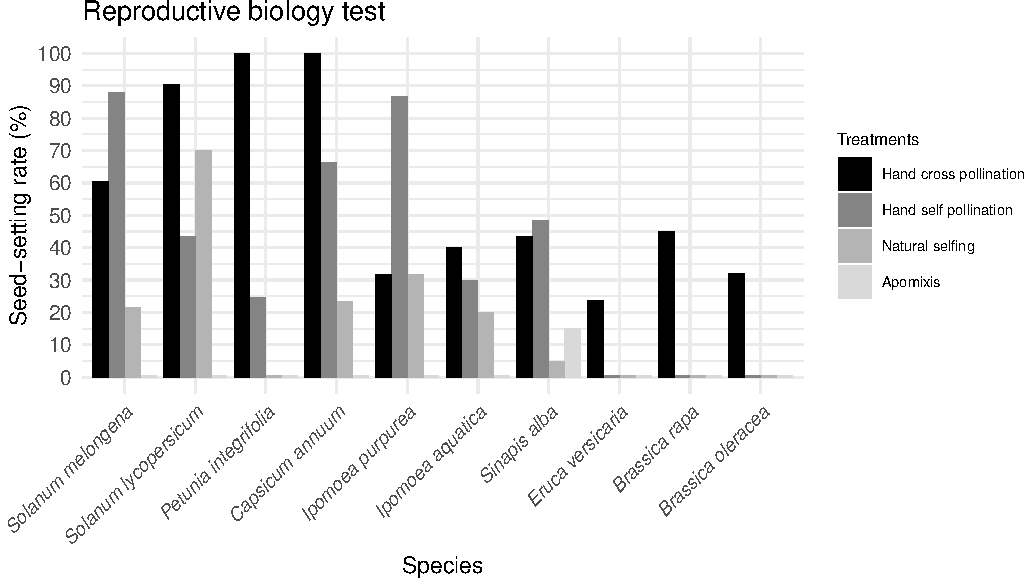
\includegraphics{output/figures/unnamed-chunk-3-1.pdf}
\caption{The effect of heterospecific pollen (scaled see set) is
represented in function of the compatibility system (self/cross*100) for
the the different species. Each coulored dot represents the interaction
of a focal species with a different pollen donor.}
\end{figure}

\newpage

\section{DISCUSSION}\label{discussion}

Discussion

What are the implications of the findings?

Ideas about pollen size in heterospecific pollen effect. (still have to
develop it more\ldots{})

Let's classify pollen size in three groups in order to understand the
interaction between pollen donor and recipient: 1) Donor pollen size
\textless{} Recipient pollen size 2) Donor pollen size = Recipient
pollen size 3) Donor pollen size \textgreater{} Recipient pollen size

Now I try to develop each part

\begin{enumerate}
\def\labelenumi{\arabic{enumi})}
\tightlist
\item
  Donor pollen size \textless{} Recipient pollen size
\end{enumerate}

Effect:

\begin{itemize}
\item
  Donor's pollen could clogg the stigma
\item
  Chemical inhibition
\end{itemize}

Traits associated with bigger pollen of the recipient:

\begin{itemize}
\item
  Recipient's pollen have faster pollen tube growth (example with my
  data)
\item
  Reduction in number of ovules (Also with my species)
\item
  Big differences in pollen size can be traduced in low relatednes
  therefore less likely of pollen germination on a far related stigma.
\end{itemize}

\begin{enumerate}
\def\labelenumi{\arabic{enumi})}
\setcounter{enumi}{1}
\tightlist
\item
  Donor pollen size = Recipient pollen size
\end{enumerate}

\begin{itemize}
\item
  Very relatedness dependant this point
\item
  Similar probabilities of taken space on the stigma
\end{itemize}

\begin{enumerate}
\def\labelenumi{\arabic{enumi})}
\setcounter{enumi}{2}
\tightlist
\item
  Donor pollen size \textgreater{} Recipient pollen size
\end{enumerate}

Effect:

-In small stigmas big pollen grains can occupy great part of the
stigmatic area.

-small pollen grains can get embeded

\emph{Negative}

-Stigma clogging

\begin{itemize}
\item
\end{itemize}

\section{CONCLUSIONS}\label{conclusions}

\section{ACKNOWLEDGEMENTS}\label{acknowledgements}

\section{REFERENCES}\label{references}

\hypertarget{refs}{}
\hypertarget{ref-aizen2007}{}
Aizen, M. A., and L. D. Harder. 2007. Expanding the limits of the
pollen-limitation concept: Effects of pollen quantity and quality.
Ecology 88:271--281.

\hypertarget{ref-arceo2016}{}
Arceo-Gómez, G., and T.-L. Ashman. 2016. Invasion status and
phylogenetic relatedness predict cost of heterospecific pollen receipt:
Implications for native biodiversity decline. Journal of Ecology
104:1003--1008.

\hypertarget{ref-ashman2013}{}
Ashman, T.-L., and G. Arceo-Gómez. 2013. Toward a predictive
understanding of the fitness costs of heterospecific pollen receipt and
its importance in co-flowering communities. American Journal of Botany
100:1061--1070.

\hypertarget{ref-barrett1988}{}
Barrett, S. C. 1988. The evolution, maintenance, and loss of
self-incompatibility systems. Plant reproductive ecology: patterns and
strategies:98--124.

\hypertarget{ref-bartomeus2008}{}
Bartomeus, I., J. Bosch, and M. Vilà. 2008. High invasive pollen
transfer, yet low deposition on native stigmas in a carpobrotus-invaded
community. Annals of Botany 102:417--424.

\hypertarget{ref-bascompte2003}{}
Bascompte, J., P. Jordano, C. J. Melián, and J. M. Olesen. 2003. The
nested assembly of plant--animal mutualistic networks. Proceedings of
the National Academy of Sciences 100:9383--9387.

\hypertarget{ref-carvalheiro2014}{}
Carvalheiro, L. G., J. C. Biesmeijer, G. Benadi, J. Fründ, M. Stang, I.
Bartomeus, C. N. Kaiser-Bunbury, M. Baude, S. I. Gomes, V. Merckx, and
others. 2014. The potential for indirect effects between co-flowering
plants via shared pollinators depends on resource abundance,
accessibility and relatedness. Ecology letters 17:1389--1399.

\hypertarget{ref-engel2003}{}
Engel, E. C., and R. E. Irwin. 2003. Linking pollinator visitation rate
and pollen receipt. American Journal of Botany 90:1612--1618.

\hypertarget{ref-fang2013}{}
Fang, Q., and S.-Q. Huang. 2013. A directed network analysis of
heterospecific pollen transfer in a biodiverse community. Ecology
94:1176--1185.

\hypertarget{ref-inouye1980}{}
Inouye, D. W. 1980. The terminology of floral larceny. Ecology
61:1251--1253.

\hypertarget{ref-lloyd1992}{}
Lloyd, D. G., and D. J. Schoen. 1992. Self-and cross-fertilization in
plants. i. functional dimensions. International Journal of Plant
Sciences 153:358--369.

\hypertarget{ref-montgomery2012}{}
Montgomery, B. R., and B. J. Rathcke. 2012. Effects of floral
restrictiveness and stigma size on heterospecific pollen receipt in a
prairie community. Oecologia 168:449--458.

\hypertarget{ref-morales2008}{}
Morales, C. L., and A. Traveset. 2008. Interspecific pollen transfer:
Magnitude, prevalence and consequences for plant fitness. Critical
Reviews in Plant Sciences 27:221--238.

\hypertarget{ref-R_Core_Team_2018}{}
R Core Team. 2018. R: A language and environment for statistical
computing. R Foundation for Statistical Computing, Vienna, Austria.

\hypertarget{ref-thomson1982}{}
Thomson, J. D., B. J. Andrews, and R. Plowright. 1982. The effect of a
foreign pollen on ovule development in diervilla lonicera
(caprifoliaceae). New Phytologist 90:777--783.

\hypertarget{ref-tong2016}{}
Tong, Z.-Y., and S.-Q. Huang. 2016. Pre-and post-pollination interaction
between six co-flowering pedicularis species via heterospecific pollen
transfer. New Phytologist 211:1452--1461.

\hypertarget{ref-whitehead2018}{}
Whitehead, M. R., R. Lanfear, R. J. Mitchell, and J. D. Karron. 2018.
Plant mating systems often vary widely among populations. Frontiers in
Ecology and Evolution 6:38.

\eleft

\clearpage

\listoftables

\newpage

\newpage

\clearpage

\listoffigures

\newpage

\newpage

\blandscape

\elandscape

\clearpage

\end{document}